\documentclass[12pt]{article}

\usepackage{artigo-muv}

\usepackage{graphicx,url}

\usepackage[brazilian]{babel}
\usepackage[utf8]{inputenc}
\usepackage[T1]{fontenc}


%\usepackage[brazil]{babel}   
%\usepackage[latin1]{inputenc}


\sloppy

\title{MUV - Mais Um Voo, Simulador para Estimar Atrasos Conforme Fluxo de
  Passageiros no Aeroporto de Guarulhos}

\author{Miguel Antonioo Copatti\inst{1},Roger Wesler Grabin\inst{2}, Anderson Seiji Ishiii\inst{3}}

\address{Escola do Mar, Ciência e Tecnologia\\
  Universidade do Vale do Itajaí (UNIVALI)\\
  Caixa Postal 360 -- 88302-202 -- Itajaí -- SC -- Brazil
%\nextinstitute
  %PEGAR E-MAIL DOS PARÇAS
  \email{miguel\_copatti@live.com,\{roger.grabing,a.ishii66\}@gmail.com}
  %\email{\{nedel,flavio\}@inf.ufrgs.br, R.Bordini@durham.ac.uk,
  %jomi@inf.furb.br}
}
\begin{document} 

\maketitle

\begin{abstract}
  %TRADUZIR RESUMO
  This meta-paper describes the style to be used in articles and short papers
  for SBC conferences. For papers in English, you should add just an abstract
  while for the papers in Portuguese, we also ask for an abstract in
  Portuguese (``resumo''). In both cases, abstracts should not have more than
  10 lines and must be in the first page of the paper.
\end{abstract}
     
\begin{resumo} 

  %contexto do trabalho 1 paragrafo
  %objetivo geral 1 paragrafo
  %apresentar metodologia 1 a 2 paragrafos
  %apresentar principais resultados 1 a 2 paragrafos 

  este meta-artigo descreve o estilo a ser usado na confeco de artigos e
  resumos de artigos para publicao nos anais das conferncias organizadas
  pela SBC. solicitada a escrita de resumo e abstract apenas para os artigos
  escritos em portugus. Artigos em ingls devero apresentar apenas abstract.
  Nos dois casos, o autor deve tomar cuidado para que o resumo (e o abstract)
  no ultrapassem 10 linhas cada, sendo que ambos devem estar na primeira
  pgina do artigo.
\end{resumo}


\section{Introdução}

%Apresentar o contexto de aplicação: do que se trata e que outros
%lugares/universidades/pesquisas também encaram este problema (1 a 2
%parágrafos)
  Atuamente o aeroporto internacional de Guarulhos ostenta o título de maior
  aeroporto do Brasil. Sua capacidade total de embarque e de desembarque é
  de 15.352 considerando todos voos, domésticos e internacionais (GRU Airport, 2018).
  A maior movimentação ocorre no terminal 3 (internacional) onde o fluxo  é de
  8.333 passageiro/hora. Contudo a capacidade de passageiro/hora pode ser 
  afetada pela quantidade de aeronaves estacionadas no pátio do terminal
  aeroportuário. Mesmo em tempo de recessão em 2017 o aeroporto registrou 
  aumento de 3,2\% se comparado com os dados de 2016. O Aeroporto planeja
  aumento no volume de passageiros e espera receber 60 milhões passageiro/ano,
  frente ao 36,6 milhões registrados no ano anterior. Para isso seja possível,
  será construído um novo pátio para aeronave e um novo pier até 2021 para o 
  terminal 3, (Aero Mgazine, 2013).

  Desde da sua inauguração no ano 1985, com uma área de 14 km quadrado,
  obteve uma movimentação de pessoas estimada em  37 milhões de passageiras
  com uma lotação total cerca de 40 milhões de aviões. Portanto observa-se
  que a capacidade máxima de passageiros será alcançada em um momento de
  pico, ocasionado por atrasos imprevistos ou datas comemorativas
  \cite{Moser:07}.
  
  % Fundamentar aspectos de Modelagem/Conceitos de Trabalhos similares e de
%estratégias utilizadas na elaboração do trabalho



%Apresentar o objetivo geral do artigo;
Este trabalho tem por objetivo coletar, avaliar e mensurar o tempo médio
entre uma aterrissagem e  decolagem de cada avião no aeroporto de guarulhos, obtendo assim alguns parâmetros para a simulação computacional, funcional do aeroporto com sua infraestrutura atual.
Posteriormente será  aplicada mudanças nas variáveis quantitativas, 
alterando.

mostrando assim um procedimento ou melhoria destinada  a população dos
estados do Brasil, principalmente do estado SP assim como de outros países,
para que não enfrentam congestionamentos ou cancelamentos de voos dada a 
densidade populacional e a quantidade de aviões.

O terceiro objetivo deste trabalho é medir a satisfação dos clientes, dada
a localização, ou seja a satisfação dos clientes no aeroporto de guarulhos, seja pela quantidade de voos ou se teve atrasos ou não.
Essa satisfação será calculada de acordo com o pouso ou e a decolagem com 
seu respectivo atraso, preço da passagem, entrega e devolução da bagagem
e também será observada o nível de contentamento dos clientes com o espaço
do aeroporto, como por exemplo, praça a alimentação, comércio, 
infraestrutura interna como por exemplo ar-condicionado, bancos, toaletes,
etc.


%verificar esse trexo
Este artigo é estruturado da seguinte maneira: a Seção 2 apresenta alguns trabalhos
relacionados a este, apontando algumas das abordagens discutidas na literatura,
em seguida, a Seção 3 apresenta a metodologia e técnicas utilizadas para a construção 
do simulador e seus artefatos produzidos neste trabalho, a Seção 4 descreve e analisa 
os resultados obtidos através da utilização do simulador, por fim, a seção 5 e última 
discute sobre algumas conclusões extraídas a partir dos resultados coletados e da 
análise do simulador, objetivos atingidos e melhorias para o simulador.
  

\section{Revisão bibliográfica} \label{sec:revisaobibliografica}

A diferença crescente entre a demanda prevista e o número de
operações efetivamente realizadas impõe aos usuários
restrições de oferta de voos pelas companhias aéreas que,
impedidas de aumentar suas frequências em Congonhas, são 
obrigadas a criar novos voos partindo de outros aeroportos,
como Guarulhos e Campinas \cite{boulic:91}.

Em contrapartida, a ANAC vem adotando medidas de restrição 
de tráfego cada vez mais severas em Congonhas, tais como: 
alocação de slots para operações, proibição de operação de 
aeronaves comerciais na pista auxiliar e determinação de tempo
máximo de permanência de aeronaves nos boxes de estacionamento,
entre outras\cite{Medau:09}. 







\section{Metodologia}

Utilizando da simulação discreta para modelar o problema afim de estimar
quando ocorre maior demanda por voos no aeroporto de Guarulhos, seja por
fatores externos, como alta demanda de passageiros, fatores climaticos,
objetos na pista, entre outros tipos de eventos que podem gerar algum 
tipo de atraso no aeroporto.


\subsection{FlightRadar24h}


%gráfico com saída dos avioes
\begin{figure}[ht]
  \centering
  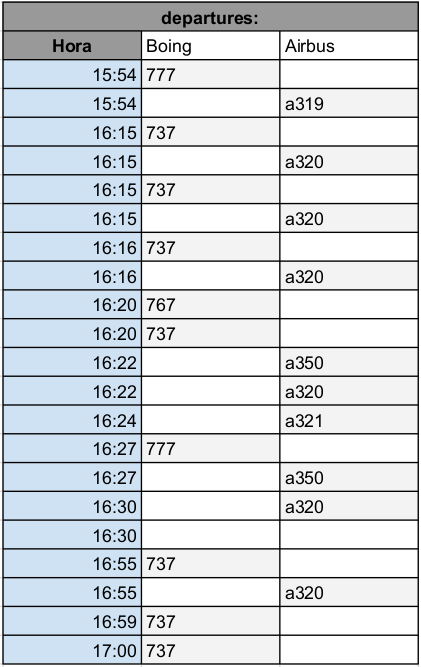
\includegraphics[width=.3\textwidth]{decolagem.png}
  \caption{Saída}
  \label{fig:saida}
\end{figure}

O  FlightRadar24 é um site e aplicativo mobile que disponibiliza a
visualização de aviões do mundo todo, em tempo real, através de mapas 
fornecidos pela Google.

Foi análisado e coletado dados, na segunda-feira e terça-feira (25 e 26 de junho), durante 
o periodo da tarde, durante pelo menos 1 hora, diariamente foi analisado 21
aeronaves saindo (decolagem) 22 aeronaves chegando (aterrisando), foi desconsiderado voos do 
tipo privado, esses que não podem ser comprado uma passagem por qualquer
individuo num aeroporto.

Durante o levantamento de dados para a modelagem do sistema, nota-se que grande parte
da frota de aeronaves são Airbus a320 e Boeing 373, que são considerados avioes de média
capacidade, limitadoa a 120 a 220, passageiros e o Boeing 373 85 até 215 passageiros 
dependendo do tipo de configuração, versão e quantidade de classes na aeronave.

Foi observado também aeronaves maiores com capacidade acima de 300 passageiros, porém 
foi um número muito pequeno e apenas voos internacionais usam esse tipo de aeronave.

%gráfico com chegada dos avioes
\begin{figure}[h!]
  \centering
  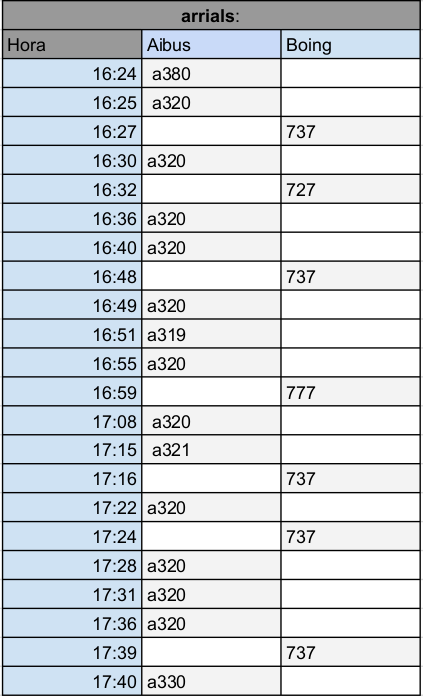
\includegraphics[width=.3\textwidth]{aterrisagem.png}
  \caption{Chegada}
  \label{fig:chegando}
\end{figure}



\section{Configuração do aeroporto}

%essa imagem nao quer ficar apos o texto [H] não funcione nem h!
% b fica na parte inferior da página
\begin{figure}[b!]
  \centering
  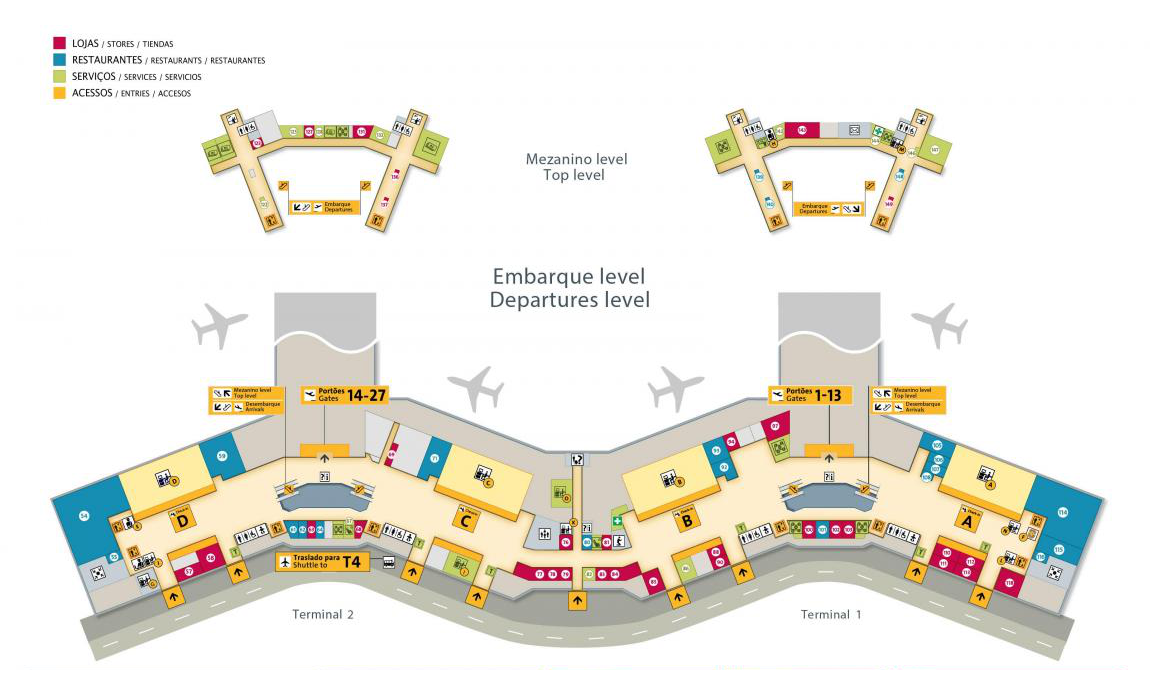
\includegraphics[width=.9\textwidth]{aeroporto.png}
  \caption{Planta geral do aeroporto de Guarulhos}
  \label{fig:aeropoto}
\end{figure}

A configuração do sistemas de pistas em geral, o fator mais importante
para determinar a capacidade de um aeroporto , sendo que o mais comum 
gargalo do sistema aeroportuário como um todo . Quando capacidade do 
sistema de pistas é excedido , o aeroporto invariavelmente começa a 
sofrer atrasos.



Atualmente o aeroporto de Guarulhos possui 2 pistas , a primeira foi 
inaugurada em 1985 com  3000 metros , a segunda possui 3500 metros, 
mais tarde ampliada para 3700 metros , há ainda previsto uma terceira
pista com extensão de 1500 metros, porém ainda não foi construída. 


\section{Definição de Capacidade e atrasos}

A eficácia de um sistema de transporte é a capacidade e a eficiência de
se processar uma unidade sendo transportada Ao passo de que o desempenho
do sistemas depende de componentes , avalia-se de forma individual cada
um deles para que seja possível determinar o resultado do sistema como 
um todo. 

Existem duas formas mais comuns de se tratar a capacidade. A primeira delas
é denominada capacidade prática que pode ser entendida como o número de 
operações de aeronaves durante um intervalo de tempo, correspondente a um
nível tolerável de atraso médio. A segunda é chamada de capacidade última,
que é a capacidade máxima ou máxima taxa de processamento. Pode ser 
definida como o número máximo de aeronaves que um aeródromo pode acomodar
durante um específico intervalo de tempo, quando submetido a uma demanda
contínua de serviço. Uma demanda contínua significa que há sempre uma 
aeronave pronta para pouso ou decolagem. 

Em termos práticos , quando duas ou mais aeronaves necessitam utilizar ao
mesmo tempo a mesma infra-estrutura, resultará em pelo menos uma aeronave 
ter que esperar, incorrendo em atraso. O atraso pode ser calculado em termos
de minutos médio de espera por aeronave chegando ou partindo em condições 
de Voos por instrumento ou voo visual. Durante os períodos de pico a demanda
pode exceder a capacidade , o que provocará a formação de filas. São raros
os casos em que a aeronave realiza um voo em perfeita e contínua sequência,
sem nenhum atraso. 

\subsection{Fatores que podem afetar a capacidade e atraso}

Os principais fatores que implicam atrasos nos aeroportos são:

%list

\begin{enumerate}
  
  \item Configuração do aeroporto: configuração geométrica relativa das pistas 
    em uso.

  \item Picos de demanda: períodos do dia em que a demanda de tráfego é muito
    alta.

  \item Composição de frota: proporção entre os tipos de aeronave que operam no 
  aeroporto, classificadas principalmente por peso e envergadura.

  \item Meteorologia: condições climáticas no aeroporto e a tecnologia de 
  instrumentação disponíveis

\end{enumerate}


\section{Detalhes do Simulador}


Figure and table captions should be centered if less than one line
(Figure~\ref{fig:exampleFig1}), otherwise justified and indented by 0.8cm on
both margins, as shown in Figure~\ref{fig:exampleFig2}. The caption font must
be Helvetica, 10 point, boldface, with 6 points of space before and after each
caption.

\begin{figure}[ht]
\centering
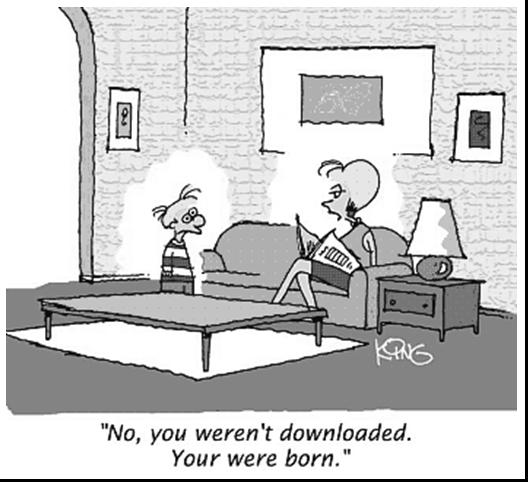
\includegraphics[width=.5\textwidth]{fig1.jpg}
\caption{A typical figure}
\label{fig:exampleFig1}
\end{figure}

\section{Modelagem e simulação}

Conforme Bateman, 2013, Simulação é uma ferramenta poderosa no 
desenvolvimento de sistemas mais eficientes, como por exemplo um simulador.

A melhoria de produtividade passou de desejo a necessidade, num mundo cada 
vez mais marcado pela globalização de mercados e pela velocidade da
tecnologia da informação, onde as empresas vencedoras são aquelas que
respondem de forma rápida e flexível às necessidades de seus clientes.
Simulação é uma ferramenta poderosa no desenvolvimento de sistemas mais
eficientes. Através dela podemos construir modelos e reconfigurar
sistemas reais em questão de dias. Esta obra apresenta fundamentos de
modelagem a processos contínuos (Bateman, 2013).

A melhoria de produtividade passou de desejo a necessidade, num mundo 
cada vez mais marcado pela globalização de mercados e pela velocidade
da tecnologia da informação, onde as empresas vencedoras são aquelas
que respondem de forma rápida e flexível às necessidades de seus clientes. 


Através dela podemos construir modelos e reconfigurar sistemas
reais em questão de dias. Esta obra apresenta fundamentos de modelagem 
a processoscontínuos, (Bateman, 2013)


Modelo é uma abstração da realidade , uma representação adaptada de acordo
com o problema a ser analisado . O objetivo da simulação não é reproduzir
a realidade em todos os aspectos, o que seria quase inviável, mas sim 
considerar aspectos relevantes a um sistemas determinado. Pode-se dizer
também que simulação é o processo de elaborar um modelo de um sistema
real e conduzir experimento, com o proposito de compreender o comportamento
e/ou avaliar várias estratégias para a operação do mesmo. Desta forma a
simulação traz vantagens como:

\begin{enumerate}

\item Possibilidade de Testar novos procedimentos operacionais, tomadas
 de decisões, estratégias de uso de pista de pouso e de rolamento, ou seja,
 podem ser avaliadas novas estratégias sem comprometer ou intervir nas 
 operações do aeroporto.

\item Possibilidade de testar possíveis configurações de pista de pouso
  pista de rolamento e terminais do aeroporto antes mesmo de sua construção, 
  bem como alterações nos arranjos físicos existentes (novas pistas de pouso
  e rolamento, terminais entre outros), antes do emprego de recursos para
  sua implantação.

\item Identificação de gargalos do sistemas , verificando quais são os 
  subsistemas, componentes ou processos que limitam o sistemas como um
  todo.

\item Compreensão de quais variáveis são mais importantes para a capacidade
e como essas variáveis interagem.

\paragraph{}%position\
Deve-se tomar cuidado com os dados obtidos na analise, pois o resultado 
da simulação nunca será igual a realidade. Uma boa analise requer 
treinamento especializado , qualidade do modelo e capacidade do analista.

\end{enumerate}

\section{Ferramenta de Simulação}

Para simulação será utilizada a Engine unity 3D, ele conta com um motor 
gráfico potente e possui um tempo de aprendizagem relativamente baixa.

Outros recursos importantíssimos ela possui, como por exemplo a física, 
\textit{pathfind} entre outros. Uma coisa que vale destacar é que a unity
tem \textit{Assets store} que contém scripts, animação, entre outros.

A principal motivação é que a \textbf{unity3D} tem sua programação já
modelada em agentes.

\bibliographystyle{sbc}
\bibliography{artigo-muv}

\end{document}
